\section{Homomorphic Encryption}

Cryptography is the practice and study of techniques for secure communication in the presence of third parties called adversaries. In its simplest form it is made up of a cryptographic function $f(\cdot)$, that can be inverted but only if you have the right key. Therefore, using a correct pair of public and secret keys, we have that $f^{-1}(f(n))=n$ for each n on which $f(\cdot)$ is defined. Traditional cryptography does not allow any operation to be performed on the encrypted data $f(n)$, otherwise you lose the original information. Homomorphic cryptography, on the other hand, is able to preserve both the additive and multiplicative structure of the integers. That is, given two integers $a$ and $b$, the following equations are valid:

\begin{align*}
  f^{-1}(f(a)+f(b)) &= a+b\\
  f^{-1}(f(a)*f(b)) &= a*b
\end{align*}

The use of these two operations, sum and product, allows us to make encrypted predictions starting from the encrypted data in input.

\subsection{The FV algorithm}

The algorithm described in the paper and used in the original CryptoNets project is YASHE, contained in the software library called SEAL \cite{dowlin2016cryptonets}. But in the meantime the library has been updated. The version that we use is v2.3, in which the algorithm implemented is a variant of the Fan-Vercauteren (FV) scheme \cite{seal-manual}. Here we present the basic version of the FV algorithm, and then we will discuss the particular version coded inside the SEAL library.

The FV scheme is an isomorphism between polynomial rings. A polynomial ring $R^a_b$ is the space consisting of all polynomials reduced modulo $x^a+1$, where the coefficients are reduced modulo $b$, ie $R^a_b = \mathbb{Z}_b[x]/(x^a+1)$. In particular, the scheme takes the polynomials from the ring $R^n_t$ as input and transforms them into an array of polynomials, each of them belonging to $R^n_q$. The polynomial array has a minimum size of 2, but increases each time a homomorphic multiplication is performed. It is possible however to subsequently reduce the size of the array (up to a minimum of 2) using a process called relinearization.

The algorithm randomly generates the polynomial $s$ in $R^n_2$: it constitutes the private (or secret) key. We will denote by $a \leftarrow R^b_c$ that $a$ has been generated with a uniform distribution from the polynomial ring $R^b_c$, and with $a \leftarrow X$ that $a$ has been generated with a truncated Gaussian distribution in the space $X$, so $s \leftarrow R^n_2$. The public key is the array $(\text{p}[0], \text{p}[1]) = ([-(as + e)]_q, a)$, with $a \leftarrow R^n_q$, and $e \leftarrow X$. The cryptographic scheme provides also the use of some special keys, called evaluation keys, to carry out the relinearization operation. The number of evaluation keys is equal to $l + 1$, with $l=\lfloor \log_w q \rfloor$ and $w$ parameter of the algorithm. Each evaluation key is composed of an array of two elements, so the $i$-th key is given by: $\text{evk}[i] = ([-(a_is+e_i)+w^is^2]_q, a_i)$, where $a_i \leftarrow R^n_q$, $e_i \leftarrow X$.

A message m $\in R^n_t$ is encrypted by computing

\begin{equation*}
    \text{c} = \left(\left[\left \lfloor \frac{q}{t} \right \rfloor m + \text{p}[0] u + e_1 \right]_q , [\text{p}[1] u + e_2 ]_q\right) 
\end{equation*}

\noindent where $u \leftarrow R^n_2$, and $e_1, e_2 \leftarrow X$. Decrypting is done by computing

\begin{equation*}
    \text{m} = \left[\left\lfloor  \frac{t}{q}  [\text{c}[0] + \text{c}[1] s]_q  \right\rceil\right]_t
\end{equation*}

Two ciphertexts $\text{c}_1$ and $\text{c}_2$ can be added together in $R^n_q$ like this:

\begin{equation*}
    \text{c}'=(\text{c}_1[0] + \text{c}_2[0], \text{c}_1[1] + \text{c}_2[1])
\end{equation*}

Multiplication is more complicated. First we calculate a new array of 3 elements like this:

\begin{align*}
    &\text{c}[0] = \left[\left\lfloor\frac{t}{q}\text{c}_1[0]\text{c}_2[0]\right\rceil\right]_q\\
    &\text{c}[1] = \left[\left\lfloor\frac{t}{q}(\text{c}_1[0]\text{c}_2[1]+\text{c}_1[1]\text{c}_2[0])\right\rceil\right]_q\\
    &\text{c}[2] = \left[\left\lfloor\frac{t}{q}\text{c}_1[1]\text{c}_2[1]\right\rceil\right]_q
\end{align*}

Then the relinearization process is performed:

\begin{align*}
    &\text{c}'[0] = \text{c}[0]+\sum\limits_{i=0}^l\text{evk}[i][0](\text{c}[2])^{(i)}\\
    &\text{c}'[1] = \text{c}[1]+\sum\limits_{i=0}^l\text{evk}[i][1](\text{c}[2])^{(i)}
\end{align*}

For more details on the FV algorithm, it is possible to consult \cite{Fan2012SomewhatPF}.

\subsection{Mismatch between data type}

As is evident at first sight, there is a problem of incompatibility between the type of data processed by a neural network and the type of data processed by the homomorphic algorithm. The first of them works with floating-point numbers, while the second one is basically a transformations between polynomials. Before seeing how the neural network works, we must therefore discuss the encoding we shall use. The SEAL library already offers the possibility of transforming a real number into a polynomial, but this method is very inefficient, because much of the polynomial is wasted. As we will see later, the Chinese remainder theorem applied to the polynomials allows us to encode in a single polynomial several different integers, which will be manipulated in parallel and all in the same way. This allows us to use less polynomials in total, and to make computation faster. The idea is therefore to use a polynomial of degree $n$ to encode $n$ values, where each value is taken from a different input, but relative to the same position in the data input structure. For example we construct the polynomial "first pixels" using the values taken from the first pixel of each of the $n$ images. Then we do the same for the "second pixels" polynomial, the "third pixels" polynomial, and so on, until all the input data have been encoded. This technique is called CRT batching. It is therefore necessary that the data to be transformed into polynomials are integers modulo $t$. To do this it is possible to perform a pre-encoding phase, in which the data are multiplied by a constant (that we call precision), rounded and reduced modulo $t$. It is also necessary to carry out the same procedure on the weights of the neural network (more details on this will be presented in the Section 3.3). The precision parameter chosen to multiply the data affects the entire computation. There is a trade-off between the accuracy of the transformed neural network, and the chosen size of the parameter $t$. $t$ in turn has a trade-off: it must be large enough so that during the entire calculation process no number exceeds $t/2$ (see the Section 2.4: Negative numbers). But at the same time a larger $t$ implies more noise in the cryptography algorithm. In our project we chose $\text{precision} = 100$; in this way all the numbers computed are smaller than $2^{80}$, which guide us in selecting the parameters for the encryption scheme. But a choice of t such that $t>2^{80}$ makes the homomorphic algorithm unusable, unless the Chinese remainder theorem is used again, but this time for a different purpose: to factorize $t$.

\subsection{Chinese remainder theorem}

The Chinese remainder theorem is a mathematical theorem dating back to the 3rd century CE, and is widely used in the field of cryptography. It allows to break down a number into a set of smaller numbers, and to reconstruct the original number starting from that set. Moreover it allows to operate on the set of small numbers, preserving the sum and product operations, just like the homomorphic schemes. The formulation is the following: given $k$ pairwise coprime numbers $n_1, n_2, ..., n_k$, we can break down a number $x$ like this:

\begin{align*}
    &x = a_1 & (\text{mod }n_1)\\
    &x = a_2 & (\text{mod }n_2)\\
    &...\\
    &x = a_k & (\text{mod }n_k)
\end{align*}

The numbers thus obtained $a_1, a_2, ..., a_k$ can be used, together with the $k$ coprime numbers, to reconstruct the number $x$, provided that $x\in[0,N)$, where $N=n_1n_2...n_k$. To do this, we must first compute the coefficients of Bézout's identity, $r_i$ and $s_i$, such that

\begin{align*}
    r_in_i+s_i\left(\frac{N}{n_i}\right) = \text{gcd}\left(n_i, \left(\frac{N}{n_i}\right)\right) = 1 && \text{for }i=1,2,...,k
\end{align*}


\noindent where gcd is the greatest common divisor, which is equal to 1 since $n_i$ and $N/n_i$ are coprime. To do this it is possible to use the Extended Euclidean algorithm. After that, it is possible to reconstruct the starting number in this way:

\begin{align*}
    & x = \sum\limits_{i=1}^k a_i s_i \frac{N}{n_i} & (\text{mod }N)
\end{align*}

This result is very useful, if not indispensable, in this project. In the original paper, which uses the old version of SEAL, the Chinese remainder theorem is used twice for two purposes: to break down the parameter $t$, and to unify more data into a single polynomial. With "break down the parameter $t$" we means to choose a set of numbers $t_i$ such that their multiplication gives the desired $t$. Therefore, in the above diagram, $t$ corresponds to the parameter $N$, and $t_i$ corresponds to $n_i$. It is important to remember that the individual $t_i$ chosen must be pairwise coprime. This is assured since in order to use CRT batching there is a more stringent requirement on the choice of parameters $t_i$: they must be prime numbers and equal to 1 (mod $2n$). If this requirement is satisfied, then there exists an $\zeta \in \mathbb{Z}_{t_i}$ so that we can break down the polynomial $x^n+1$ as follows:

\begin{align*}
    &x^n+1 = (x - \zeta)(x - \zeta^3)...(x - \zeta^{2n-1}) & (\text{mod }t_i)
\end{align*}

Therefore it is possible to decompose the polynomial ring $R^n_{t_i}$ into $n$ spaces $\mathbb{Z}_{t_i}$:

\begin{equation*}
    R_{t_i} \cong \prod \limits_{i=0}^{n-1} \mathbb{Z}_{t_i}
\end{equation*}

This is the procedure underlying CRT batching. More details are shown in \cite{seal-manual}.

As we mentioned before, the version of SEAL used in our project is v2.3, which uses a variant of the FV algorithm described above. In particular, in our version of the software library the theorem is used on three occasions, two of which correspond to those of the original paper, described above. The third and new use of the theorem lies in the decomposition of the parameter $q$ into smaller numbers. Also in this case we mean to break down the parameter $q$ with a set of numbers $q_i$ such that $q_1q_2...q_i = q$. This is a variant of the cryptographic scheme which is not present in the original FV algorithm \cite{Fan2012SomewhatPF}. Due to this fact, the parameter $q$ differs between the two SEAL versions. In the original CryptoNets project, the researchers used 192 bits to represent $q$. We instead use 4 numbers, all between 55 and 60 bits, whose product gives a 230 bit number. So our project has a slightly larger $q$
, which slightly decreases the noise produced by the cryptographic algorithm.

\subsection{Negative numbers}

A final consideration concerning the use of the cryptographic scheme is given by the problem of negative numbers. The data manipulated by the neural network are always reduced modulo $t$, even when they are encrypted. Which means that at any time of the computation in the neural network, if you decrypt the output of a layer and recompose its values with the inverse of CRT batching, each resulting number will be an integer between 0 and $t$ ($t$ excluded). This can be a problem, as the original neural network, in addition to presenting floating-point numbers, also manipulate negative numbers. It can happen, in fact, that in the final layer there are negative numbers which, once reduced modulo $t$, become positive. Because now they're positive, these numbers can influence the choice of the final class for a certain input. In fact, at the end of the neural network computation, the prediction is given by choosing the class associated with the highest value among those present in the output neurons. It is therefore possible that one of those values which, in the original neural network, would have been negative and not chosen, is chosen. To avoid this problem, we need to find a way to encode negative numbers within the space of integers $[0, t)$. To do this, we use the following scheme:

\begin{figure}[H]
	\centering
	\makebox[\columnwidth]{
		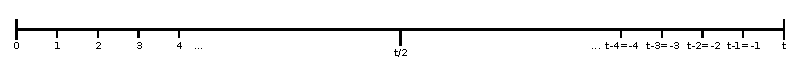
\includegraphics[width=0.8\paperwidth]{images/fig1.pdf}
	}
    \caption{Encoding of negative numbers in the $[0,t)$ span.}
    \label{fig:im1}
\end{figure}

\noindent so we divide the set $[0, t)$ into two parts: the first part contains only the positive numbers, while the second part contains only negative numbers. This is because given a negative number $-n$, its reduction modulo $t$ is equal to $t-n$. To do this, and to avoid that the two sub-sets overlap, it is therefore mandatory that no number during the computation of the neural network, taken as an absolute value, exceeds half of $t$: $\forall  n, |n|<t/2$. This allows us to reconstruct the output, after using the Chinese remainder theorem, using the following algorithm:

\lstset{frame=tb,
  language=Python,
  breaklines=true,
  showstringspaces=false,
  columns=flexible,
  numbers=none,
  tabsize=3,
  escapeinside={(*@}{@*)}
}

\begin{lstlisting}[frame=single]
n = crt_inverse(array)
negative_threshold = t / 2
if n > negative_threshold:
    n = n (*@-@*) t
\end{lstlisting}
